\chapter{L'organisation des systèmes nerveux}\label{ch:b3:nervous-systems}

Une méduse a quelques milliers de neurones en un réseau sans centre et
sait nager, se nourrir et se redresser. Une pieuvre en a un demi-milliard,
les deux tiers dans ses bras, dont chacun sait résoudre un problème dont
le cerveau n'a rien su. Vous en avez quatre-vingt-six milliards, joints
par cent mille milliards de synapses, tournant sur vingt watts --- un
cinquième de votre énergie pour deux pour cent de votre masse --- et
Santiago Ramón y Cajal, les dessinant cellule par cellule dans les
années 1890 à partir de coupes imprégnées d'argent, vit qu'il s'agissait
de cellules séparées qui se touchaient sans fusionner et que les signaux
les traversaient dans un seul sens. Le volume précédent traitait du
neurone~: son potentiel de repos, son potentiel d'action, sa synapse. Ce
chapitre traite de ce dans quoi les neurones sont câblés~: le câble
passif qui limite la distance et la vitesse de propagation d'un signal,
les circuits --- réflexe, oscillateur, entourage inhibiteur --- dont on
assemble le comportement, le plan du système nerveux des vertébrés et
celui de la \omterm{def:b3:nervous-systems:cells}{glie} qui le fait tourner, son budget énergétique, et les
façons dont différents animaux ont réparti leurs neurones.

\section{Les neurones et la glie}

\begin{definition}[Les cellules du système nerveux]\label{def:b3:nervous-systems:cells}
\index{neurone!types}\index{glie}\index{astrocyte}\index{oligodendrocyte}\index{myéline}\index{microglie}\index{interneurone}
Les neurones se présentent en quelques architectures qui reviennent
partout dans le cerveau~: les cellules \emph{pyramidales}, neurones de
projection excitateurs du cortex, avec une longue dendrite apicale et un
axone qui peut parcourir un mètre~; les cellules de \emph{Purkinje} du
\omterm{def:b3:nervous-systems:plan}{cervelet}, dont l'arbre dendritique aplati reçoit deux cent mille
synapses~; les neurones sensoriels à un prolongement vers la périphérie
et un vers la moelle~; et les \emph{interneurones}, cellules à axone
court qui restent dans une région, inhibitrices pour la plupart. Environ
quatre neurones corticaux sur cinq libèrent du glutamate et excitent~;
un sur cinq libère du GABA et inhibe. La \emph{glie}, aussi nombreuse
que les neurones, fait le reste. Les \emph{astrocytes} enveloppent
synapses et vaisseaux sanguins~: ils captent le potassium que libèrent
les neurones qui déchargent et le glutamate que répandent les synapses,
fournissent du lactate, règlent le débit sanguin local, et induisent et
entretiennent la \omterm{prop:b3:nervous-systems:barrier-budget}{barrière hémato-encéphalique}. Les
\emph{oligodendrocytes} du système nerveux central et les \emph{cellules
de Schwann} de la périphérie enveloppent les axones de \emph{myéline},
des dizaines de couches de membrane qui isolent l'axone entre les nœuds
où siègent les canaux. La \emph{microglie} est faite des \omterm{def:b3:innate-immunity:innate}{macrophages}
résidents du cerveau, qui élaguent les synapses au cours du
développement et nettoient les débris. Les cellules épendymaires
tapissent les ventricules et fabriquent le \omterm{prop:b3:nervous-systems:barrier-budget}{liquide céphalorachidien}.
\end{definition}

\begin{proof}[Faits expérimentaux]
L'imprégnation au chromate d'argent de Golgi (1873) noircissait, pour
des raisons inconnues, environ un neurone sur cent, entièrement, en
laissant les autres invisibles --- de sorte qu'une cellule unique
pouvait être vue en entier dans un enchevêtrement de millions. Golgi
lisait ses propres préparations comme un réticulum continu~; Cajal, à
partir de 1888, en appliquant la même imprégnation à des tissus
embryonnaires où les cellules sont plus simples, vit que chaque cellule
se terminait librement, que dendrites et axone différaient, et que les
axones se terminaient sur les dendrites et les corps d'autres cellules
sans s'y joindre. De la disposition des cellules sensorielles et
motrices il déduisit le sens de l'écoulement --- dendrite, corps, axone
--- la \emph{loi de la polarisation dynamique}. Sherrington nomma
l'intervalle \emph{synapse} en 1897~; le microscope électronique le
montra en 1954.
\end{proof}

\begin{omfigure}
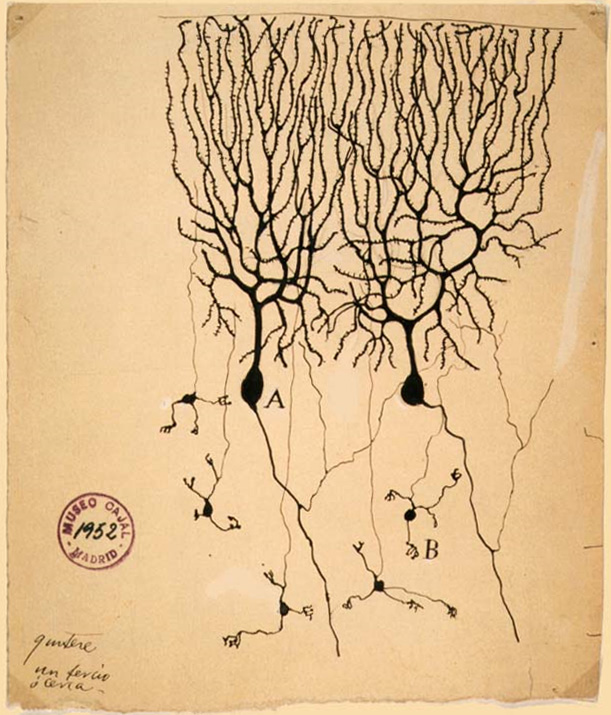
\includegraphics[width=0.30\linewidth]{images/book5/cajal-purkinje.jpg}\hspace{0.04\linewidth}
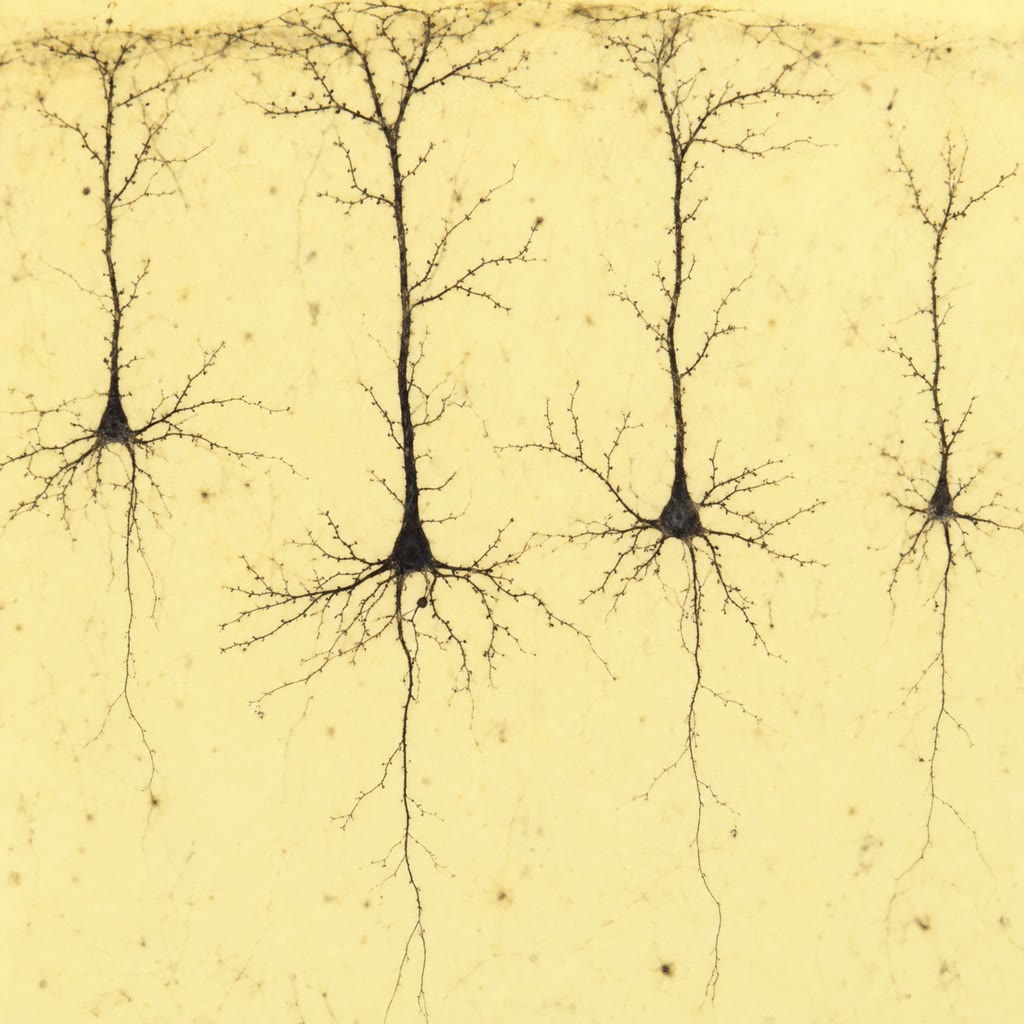
\includegraphics[width=0.30\linewidth]{images/book5/ai/b5-17-cortex-neurons.jpg}\hspace{0.04\linewidth}
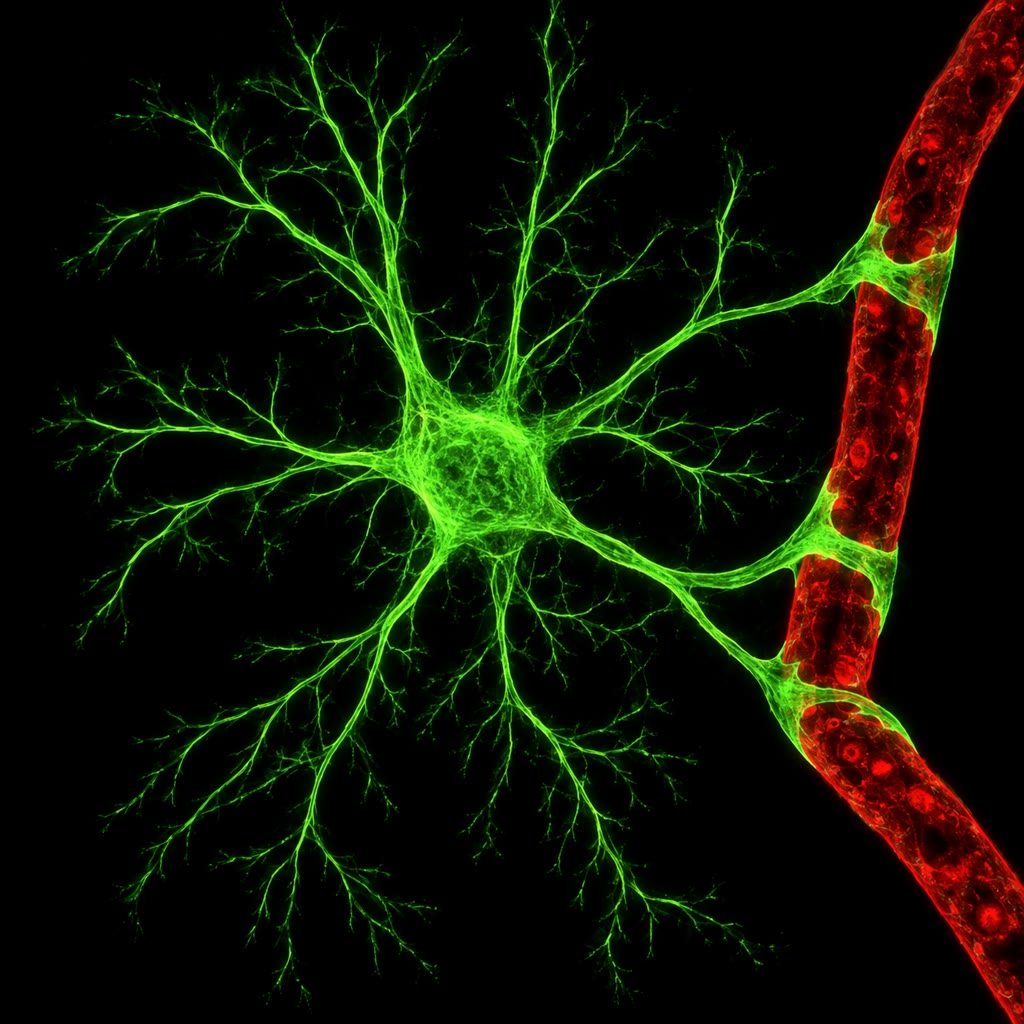
\includegraphics[width=0.30\linewidth]{images/book5/ai/b5-17-astrocyte.jpg}

{\small À gauche~: une cellule de Purkinje du \omterm{def:b3:nervous-systems:plan}{cervelet} dessinée par
Cajal (1899) d'après une coupe imprégnée par la méthode de Golgi --- tout
l'arbre dendritique d'une seule cellule, l'argument du neurone comme
unité (domaine public). Au centre~: des neurones pyramidaux du cortex en
imprégnation de Golgi. À droite~: un \omterm{def:b3:nervous-systems:cells}{astrocyte} (en vert) avec ses pieds
sur un capillaire (en rouge).}
\end{omfigure}

\section{Le neurone comme câble}

\begin{theorem}[L'équation du câble en régime stationnaire]\label{thm:b3:nervous-systems:cable}
\index{équation du câble}\index{constante d'espace}\index{constante de temps!membranaire}\index{vitesse de conduction}
Modélisons une dendrite ou un axone amyélinique par un cylindre de
diamètre $d$ dont le cytoplasme a la résistivité $R_{i}$ et dont la
membrane a la résistance spécifique $R_{m}$ (résistance fois aire) et la
capacité $C_{m}$ par aire. Par unité de longueur la résistance axiale
vaut $r_{i} = 4R_{i}/\pi d^{2}$ et la résistance membranaire
$r_{m} = R_{m}/\pi d$. Une tension constante $V_{0}$ appliquée en
$x = 0$ se propage le long de la fibre selon
\[
V(x) = V_{0}\,e^{-x/\lambda}, \qquad
\lambda = \sqrt{\frac{r_{m}}{r_{i}}} = \sqrt{\frac{R_{m}\,d}{4R_{i}}},
\]
où $\lambda$ est la \emph{\omterm{thm:b3:nervous-systems:cable}{constante d'espace}}~: la distance sur laquelle
un signal passif tombe à $1/e$, qui croît comme la racine carrée du
diamètre. La membrane se charge avec la \emph{constante de temps} $\tau =
R_{m}C_{m}$, indépendante de la géométrie. Un potentiel d'action, qui se
régénère lui-même, parcourt un axone amyélinique à une vitesse
proportionnelle à $\lambda/\tau$ et donc à $\sqrt{d}$~; le long d'un
axone myélinisé, où il saute de nœud en nœud, à une vitesse
proportionnelle à $d$ --- environ \qty{6}{m/s} par micromètre de diamètre.
\end{theorem}
\begin{proof}
Soit $I(x)$ le courant axial. La loi d'Ohm le long du cœur donne
$\mathrm{d}V/\mathrm{d}x = -r_{i}I$~; la conservation de la charge en
régime stationnaire dit que le courant axial perdu entre $x$ et
$x + \mathrm{d}x$ fuit par la membrane,
$\mathrm{d}I/\mathrm{d}x = -V/r_{m}$. En dérivant la première et en y
portant la seconde,
$\mathrm{d}^{2}V/\mathrm{d}x^{2} = (r_{i}/r_{m})V = V/\lambda^{2}$,
équation linéaire du second ordre dont la solution bornée quand
$x \to \infty$ est $V_{0}e^{-x/\lambda}$. En substituant
$r_{m} = R_{m}/\pi d$ et $r_{i} =
4R_{i}/\pi d^{2}$ on obtient $\lambda^{2} = R_{m}d/4R_{i}$. La constante
de temps est celle d'une résistance et d'un condensateur en parallèle,
$r_{m}c_{m} =
(R_{m}/\pi d)(C_{m}\pi d) = R_{m}C_{m}$. Pour les vitesses~: une onde
qui se régénère doit charger la membrane une \omterm{thm:b3:nervous-systems:cable}{constante d'espace} en avant
en à peu près une constante de temps, donc
$v \sim \lambda/\tau \propto \sqrt{d}$~; entre les nœuds d'un axone
myélinisé la membrane internodale a une résistance relevée et une
capacité abaissée par la centaine de couches de \omterm{def:b3:nervous-systems:cells}{myéline}, la longueur
internodale croît comme $d$, et le résultat est $v \propto d$. Les
constantes de proportionnalité sont admises.
\end{proof}

\begin{example}[Quelques nombres pour une dendrite et deux axones]\label{ex:b3:nervous-systems:numbers}
Une dendrite de $d = \qty{2}{\micro m}$ avec $R_{m} = \qty{2e4}{\ohm.cm^2}$
et $R_{i} = \qty{100}{\ohm.cm}$~: $\lambda = \sqrt{2\times 10^{4}\times
2\times 10^{-4}/400}\ \unit{cm} = \qty{0.1}{cm} = \qty{1}{mm}$ --- un
potentiel synaptique au bout d'une dendrite d'un millimètre atteint le
corps cellulaire au tiers de sa taille, et c'est pourquoi la géométrie
d'un arbre dendritique fait partie de son calcul. $\tau = 2\times 10^{4}\times
10^{-6}\,\unit{F/cm^2}\cdot\unit{\ohm.cm^2} = \qty{20}{ms}$, la fenêtre
dans laquelle les entrées doivent arriver pour se sommer. Un axone géant
de calmar de \qty{500}{\micro m}, amyélinique, conduit à environ
\qty{25}{m/s}~; pour en faire autant un vertébré emploie un axone
myélinisé de \qty{4}{\micro m}, quinze mille fois plus petit en section
--- la raison pour laquelle un nerf de vertébré peut porter dix mille
fibres rapides dans la place d'un seul axone de calmar. Un axone moteur
de \qty{20}{\micro m} conduit à \qty{120}{m/s}~; quand la sclérose en
plaques lui retire sa \omterm{def:b3:nervous-systems:cells}{myéline} la vitesse tombe d'un facteur dix et la
conduction peut échouer tout à fait aux endroits dénudés.
\end{example}

\begin{omfigure}
\begin{tikzpicture}
\begin{axis}[
  width=6.4cm, height=5.2cm,
  axis x line=bottom, axis y line=left,
  xmin=0, xmax=3, ymin=0, ymax=1.05,
  xlabel={distance (mm)}, ylabel={$V/V_{0}$},
  xlabel style={font=\small, at={(axis description cs:0.5,-0.12)}, anchor=north}, ylabel style={font=\small},
  tick label style={font=\scriptsize}, xtick={0,1,2,3}, ytick={0,0.37,1}, yticklabels={0,$1/e$,1},
  clip=false,
]
\addplot[very thick, omDef, domain=0:3, samples=60] {exp(-x/1.0)};
\addplot[very thick, omThm, domain=0:3, samples=60] {exp(-x/0.5)};
\node[font=\scriptsize, omDef, anchor=south west] at (axis cs:1.2,0.45) {$d = \qty{2}{\micro m}$, $\lambda = \qty{1}{mm}$};
\node[font=\scriptsize, omThm, anchor=north west] at (axis cs:0.8,0.22) {$d = \qty{0.5}{\micro m}$, $\lambda = \qty{0.5}{mm}$};
\end{axis}
\begin{axis}[
  at={(7.6cm,0)}, anchor=south west,
  width=6.4cm, height=5.2cm,
  xmode=log, ymode=log,
  xmin=0.1, xmax=1000, ymin=0.1, ymax=200,
  xlabel={diamètre de l'axone ($\unit{\micro m}$)}, ylabel={vitesse (m/s)},
  xlabel style={font=\small, at={(axis description cs:0.5,-0.12)}, anchor=north}, ylabel style={font=\small},
  tick label style={font=\scriptsize},
  clip=false,
]
\addplot[very thick, omDef, domain=1:25, samples=2] {6*x};
\addplot[very thick, omThm, domain=0.2:1000, samples=2] {1.1*sqrt(x)};
\fill[omThm] (axis cs:500,25) circle (2pt); \node[font=\scriptsize, anchor=north east] at (axis cs:500,23) {axone géant de calmar};
\fill[omDef] (axis cs:20,120) circle (2pt); \node[font=\scriptsize, anchor=west] at (axis cs:26,120) {axone moteur humain};
\node[font=\scriptsize, omDef, anchor=north west, align=left] at (axis cs:1.2,60) {myélinisé~: $v \propto d$};
\node[font=\scriptsize, omThm, anchor=north west, align=left] at (axis cs:2,0.7) {amyélinique~: $v \propto \sqrt{d}$};
\end{axis}
\end{tikzpicture}

{\small À gauche~: décroissance passive d'un signal constant le long
d'une dendrite, pour deux diamètres --- la \omterm{thm:b3:nervous-systems:cable}{constante d'espace} croît comme
$\sqrt{d}$. À droite~: la \omterm{thm:b3:nervous-systems:cable}{vitesse de conduction} en fonction du diamètre~;
la \omterm{def:b3:nervous-systems:cells}{myéline} permet à une fibre de \qty{4}{\micro m} de faire ce à quoi un
axone amyélinique aurait besoin d'un demi-millimètre.}
\end{omfigure}

\section{Les circuits}

\begin{definition}[Les circuits élémentaires]\label{def:b3:nervous-systems:circuits}
\index{arc réflexe}\index{inhibition réciproque}\index{inhibition antérograde}\index{inhibition rétroactive}\index{convergence}\index{divergence}
Un \emph{arc réflexe} est le plus court chemin d'un capteur à un
effecteur~: dans le réflexe rotulien, un afférent de fuseau
neuromusculaire entre dans la moelle et fait synapse directement sur les
motoneurones du même muscle, qui le contractent environ \qty{30}{ms}
après le coup --- une synapse, pas de cerveau. Le même afférent excite
un \omterm{def:b3:nervous-systems:cells}{interneurone} inhibiteur vers les motoneurones du muscle opposé
(\emph{inhibition réciproque}), de sorte que la contraction de
l'extenseur n'est pas combattue par le fléchisseur. La plupart des
circuits sont bâtis sur quelques motifs~: la \emph{divergence}, un
neurone en commandant beaucoup, et la \emph{convergence}, beaucoup sur
un, qui somme les indices~; l'\emph{inhibition antérograde}, où une
entrée excite à la fois une cible et un \omterm{def:b3:nervous-systems:cells}{interneurone} qui inhibe la cible
une milliseconde plus tard, ce qui affine la réponse dans le temps~;
l'\emph{inhibition rétroactive}, où la sortie de la cible elle-même
excite un \omterm{def:b3:nervous-systems:cells}{interneurone} qui l'inhibe, ce qui limite la décharge et,
étendu aux voisins, produit l'inhibition latérale qui accentue le
contraste (\cref{ch:b3:sensory-systems})~; et la \emph{désinhibition},
inhiber un inhibiteur, la façon qu'ont les noyaux gris centraux de
libérer un mouvement.
\end{definition}

\begin{omfigure}
\begin{tikzpicture}[every node/.style={font=\scriptsize}, >=stealth]
  % spinal cord cross-section (schematic)
  \draw[thick, omDef!60, fill=omDef!8] (5.4,1.5) ellipse (2.0 and 1.5);
  \draw[thick, gray, fill=gray!15] (5.4,1.5) .. controls (4.7,2.4) and (4.0,2.6) .. (4.0,1.9) .. controls (4.0,1.2) and (4.6,0.9) .. (4.8,0.5) .. controls (5.0,0.2) and (5.8,0.2) .. (6.0,0.5) .. controls (6.2,0.9) and (6.8,1.2) .. (6.8,1.9) .. controls (6.8,2.6) and (6.1,2.4) .. (5.4,1.5);
  \node[above] at (5.4,3.05) {moelle épinière};
  % muscles
  \draw[thick, omMeth!70!black, fill=omMeth!20] (0.2,0.2) rectangle (1.4,2.0); \node[below, align=center] at (0.8,0.1) {extenseur\\(quadriceps)};
  \draw[thick, omThm!70!black, fill=omThm!15] (0.2,-2.6) rectangle (1.4,-1.4); \node[below, align=center] at (0.8,-2.7) {fléchisseur\\(ischio-jambiers)};
  \fill[omProp] (0.8,1.3) ellipse (0.12 and 0.3); \node[left, font=\tiny] at (0.65,1.3) {fuseau};
  % Ia afferent to cord (dorsal)
  \draw[very thick, omProp] (0.9,1.3) .. controls (2.0,2.6) and (3.6,2.9) .. (4.8,2.2); \fill[omProp] (4.8,2.2) circle (0.09);
  \node[above, omProp] at (2.6,2.85) {afférent Ia~: étirement};
  % motor neuron to extensor
  \fill[omMeth!70!black] (5.0,0.9) circle (0.16);
  \draw[->, very thick, omMeth!70!black] (4.9,0.85) .. controls (3.4,0.3) and (2.0,0.4) .. (1.4,1.0);
  \draw[->, thick, omProp] (4.8,2.2) -- (5.0,1.1);
  % inhibitory interneuron to flexor motor neuron
  \fill[omThm] (6.1,1.7) circle (0.13);
  \draw[->, thick, omProp] (4.9,2.25) -- (6.0,1.8);
  \fill[omThm!70!black] (6.0,0.6) circle (0.16);
  \draw[-|, thick, omThm] (6.1,1.55) -- (6.0,0.8);
  \draw[->, very thick, omThm!70!black, dashed] (5.9,0.5) .. controls (4.8,-0.8) and (3.0,-1.6) .. (1.4,-2.0);
  % right-hand labels with leaders
  \node[right, omThm, font=\tiny] at (7.6,1.9) {interneurone inhibiteur Ia}; \draw[gray, thin] (7.55,1.9) -- (6.25,1.7);
  \node[right, omMeth!70!black, font=\tiny, align=left] at (7.6,1.1) {motoneurone extenseur~: excité}; \draw[gray, thin] (7.55,1.1) -- (5.15,0.9);
  \node[right, omThm!70!black, font=\tiny, align=left] at (7.6,0.3) {motoneurone fléchisseur~: inhibé}; \draw[gray, thin] (7.55,0.3) -- (6.15,0.6);
  \node[below] at (4.6,-0.15) {réflexe monosynaptique~: $\sim$\qty{30}{ms}};
  \node[below, align=center] at (4.2,-2.0) {inhibition réciproque~:\\l'antagoniste se relâche};
\end{tikzpicture}

{\small Le réflexe d'étirement. Un coup étire les fuseaux de
l'extenseur~; l'afférent Ia excite directement les motoneurones de
l'extenseur (une synapse) et, par un \omterm{def:b3:nervous-systems:cells}{interneurone} inhibiteur, fait taire
ceux du fléchisseur.}
\end{omfigure}

\begin{proposition}[Les générateurs centraux de rythme]\label{prop:b3:nervous-systems:cpg}
\index{générateur central de rythme}\index{oscillateur à demi-centres}
Les mouvements rythmiques --- respirer, marcher, nager, mâcher --- sont
produits par des circuits du \omterm{def:b3:nervous-systems:plan}{tronc cérébral} et de la \omterm{def:b3:nervous-systems:plan}{moelle épinière} qui
oscillent d'eux-mêmes, les \emph{générateurs centraux de rythme}, que la
rétroaction sensorielle ajuste mais ne crée pas~: la moelle d'un chat
séparée du cerveau et privée de ses nerfs sensoriels produit encore le
patron alterné de la marche. Le montage le plus simple est le
\emph{demi-centre} de Brown (1911)~: deux groupes de neurones qui
s'inhibent l'un l'autre. Celui qui décharge fait taire son partenaire~;
mais un groupe qui décharge se fatigue --- ses canaux s'inactivent, son
inhibition du partenaire faiblit --- et le partenaire, libéré, décharge
et fait taire à son tour le premier~: l'alternance, avec une période
fixée par la constante de temps de la fatigue et non par une horloge. Le
rythme respiratoire naît dans un amas de quelques milliers de neurones
du bulbe (le complexe pré-Bötzinger), qui décharge par bouffées de la
naissance à la mort~; la nage de la lamproie est une chaîne de
demi-centres le long de sa moelle, chacun retardé sur le précédent de
sorte qu'une onde file vers la queue.
\end{proposition}

\begin{omfigure}
\begin{tikzpicture}[every node/.style={font=\scriptsize}, >=stealth]
  % half-centre
  \begin{scope}
    \draw[thick, fill=omDef!25] (0,0) circle (0.5); \node at (0,0) {L};
    \draw[thick, fill=omThm!25] (3,0) circle (0.5); \node at (3,0) {R};
    \draw[-|, very thick] (0.5,0.2) -- (2.5,0.2); \draw[-|, very thick] (2.5,-0.2) -- (0.5,-0.2);
    \node[above] at (1.5,0.3) {inhibition mutuelle};
    \draw[->, thick, omDef] (0,-0.5) -- (0,-1.3) node[below] {muscles gauches};
    \draw[->, thick, omThm] (3,-0.5) -- (3,-1.3) node[below] {muscles droits};
    \draw[->, thick, gray] (-1.2,0.6) -- (-0.45,0.25) node[pos=0, above, align=center] {commande tonique\\du tronc cérébral};
    \draw[->, thick, gray] (4.5,0.6) -- (3.45,0.25);
  \end{scope}
  % traces
  \begin{scope}[xshift=6.0cm, yshift=0.9cm]
    \node[left, omDef] at (0,0) {L};
    \foreach \x in {0,2,4} { \foreach \s in {0.1,0.2,...,0.9} \draw[omDef] (\x+\s,-0.15) -- (\x+\s,0.15); }
    \node[left, omThm] at (0,-1.0) {R};
    \foreach \x in {1,3,5} { \foreach \s in {0.1,0.2,...,0.9} \draw[omThm] (\x+\s,-1.15) -- (\x+\s,-0.85); }
    \draw[->] (0,-1.6) -- (6.2,-1.6) node[right] {temps};
    \draw[<->] (0,-2.0) -- (2,-2.0) node[midway, below] {période~: fixée par la fatigue};
  \end{scope}
\end{tikzpicture}

{\small Un \omterm{prop:b3:nervous-systems:cpg}{oscillateur à demi-centres}. Deux groupes qui s'inhibent
mutuellement sous une commande constante alternent~: le côté actif se
fatigue, son inhibition faiblit, l'autre côté s'échappe et prend le
relais. Aucun neurone n'est lui-même rythmique.}
\end{omfigure}

\begin{method}[Tracer un circuit]\label{met:b3:nervous-systems:tracing}
\index{traçage de circuit}\index{optogénétique}
Pour établir que le neurone A commande le neurone B et que la voie
compte pour un comportement~: (1) l'anatomie --- injecter un traceur qui
chemine le long des axones (un colorant, un \omterm{def:b3:virology:virus}{virus} de la rage modifié qui
franchit une synapse à rebours) et trouver les cellules connectées~; (2)
la physiologie --- enregistrer B pendant qu'on stimule A, et mesurer la
latence (une connexion monosynaptique donne un délai fixe d'environ une
milliseconde) et le signe (excitation ou inhibition)~; (3) la nécessité
--- faire taire A, par lésion, par refroidissement, ou en y exprimant
une pompe à chlorure commandée par la lumière qu'on éclaire
(l'\emph{optogénétique}), et voir si le comportement échoue~; (4) la
suffisance --- activer A seul, avec un canal cationique commandé par la
lumière, et voir si le comportement apparaît~; (5) chez un animal
intact, imager l'activité de toute la population avec un indicateur
calcique pendant que le comportement est exécuté. Un circuit est établi
quand les cinq concordent~; la plupart des circuits publiés en ont deux
ou trois.
\end{method}

\section{Le plan du système nerveux des vertébrés}

\begin{definition}[Divisions centrale et périphérique]\label{def:b3:nervous-systems:plan}
\index{moelle épinière}\index{tronc cérébral}\index{cervelet}\index{thalamus}\index{hypothalamus}\index{cortex cérébral}\index{système nerveux autonome}\index{système nerveux entérique}
Le \emph{système nerveux central} est le cerveau et la moelle épinière~;
le \emph{périphérique} est tout le reste. La \emph{moelle épinière}
reçoit les axones sensoriels par ses racines dorsales et envoie les
axones moteurs par ses racines ventrales, sa substance grise dessinant
un papillon de corps cellulaires, sa substance blanche faite des
faisceaux myélinisés qui montent et descendent. Le \emph{tronc cérébral}
--- bulbe, pont, mésencéphale --- porte les noyaux des nerfs crâniens et
les centres qui entretiennent sans y penser la respiration, le rythme
cardiaque et la pression artérielle~; une mort du tronc cérébral est la
mort. Le \emph{cervelet}, qui a plus de neurones que tout le reste du
cerveau, règle le tempo et la coordination du mouvement et apprend de
l'erreur. Le \emph{thalamus} relaie vers le cortex tous les sens sauf
l'odorat, et les réponses du cortex en retour~; l'\emph{hypothalamus}
qui est dessous mène l'homéostasie --- température, faim, soif, horloge,
axes endocriniens du \cref{ch:b3:endocrinology}. Les \emph{noyaux gris
centraux} choisissent parmi les actions possibles~; l'\emph{hippocampe}
fabrique les souvenirs (\cref{ch:b3:learning-memory})~; et le
\emph{cortex cérébral}, feuillet de six couches de cellules épais de
deux à quatre millimètres et large d'un quart de mètre carré, plié pour
tenir, fait le reste, dans des aires cartographiées pour chaque sens et
chaque mouvement et dans les aires associatives entre elles. La division
\emph{autonome} du système périphérique mène les organes~: la chaîne
\emph{sympathique}, qui libère de la noradrénaline, mobilise (cœur
accéléré, intestin ralenti, pupilles larges)~; les nerfs
\emph{parasympathiques}, qui libèrent de l'acétylcholine, économisent et
digèrent~; et le système nerveux \emph{entérique}, un demi-milliard de
neurones dans la paroi de l'intestin, mène la digestion tout seul.
\end{definition}

\begin{omfigure}
\begin{tikzpicture}[every node/.style={font=\scriptsize}, >=stealth]
  % sagittal brain schematic
  \draw[thick, omDef!70, fill=omDef!15] (0,2.0) .. controls (0,4.6) and (3.5,5.4) .. (6.0,4.4) .. controls (7.6,3.7) and (7.4,2.2) .. (6.2,1.9) .. controls (5.4,1.7) and (5.2,1.3) .. (4.4,1.6) .. controls (3.0,1.3) and (1.2,1.4) .. (0,2.0);
  \node[align=center] at (3.0,3.9) {cortex cérébral~: six couches,\\aires sensorielles, motrices et associatives};
  % basal ganglia / hippocampus (deep)
  \draw[thick, omProp!70, fill=omProp!25] (3.2,2.6) ellipse (0.9 and 0.45); \node[font=\tiny] at (3.2,2.6) {noyaux gris centraux};
  \draw[thick, omProp!70, fill=omProp!25] (5.2,2.45) ellipse (0.88 and 0.3); \node[font=\tiny] at (5.2,2.45) {hippocampe};
  % thalamus, hypothalamus
  \draw[thick, omMeth!70!black, fill=omMeth!25] (4.0,1.95) ellipse (0.7 and 0.3); \node[font=\tiny] at (4.0,1.95) {thalamus};
  \draw[thick, omMeth!70!black, fill=omMeth!40] (4.0,1.42) ellipse (0.78 and 0.22); \node[font=\tiny] at (4.0,1.42) {hypothalamus};
  % cerebellum
  \draw[thick, omThm!70, fill=omThm!20] (6.6,1.2) ellipse (0.9 and 0.6); \node[font=\tiny] at (6.6,1.2) {cervelet};
  % brainstem
  \draw[thick, gray!70, fill=gray!20] (4.7,1.2) -- (5.5,1.2) -- (5.9,-0.3) -- (5.1,-0.3) -- cycle; \node[font=\tiny, rotate=-75] at (5.3,0.45) {tronc cérébral};
  % spinal cord
  \draw[thick, gray!70, fill=gray!20] (5.2,-0.3) rectangle (5.8,-1.6); \node[right, font=\tiny] at (5.85,-1.0) {moelle épinière};
  % labels with leaders on the right
  \node[right, align=left] at (7.8,3.4) {thalamus~: relais de tous les\\sens sauf l'odorat~; hypothalamus~:\\homéostasie, horloge, axes endocriniens};
  \draw[gray] (7.75,3.3) -- (4.7,1.95);
  \node[right, align=left] at (7.8,1.9) {cervelet~: tempo et\\coordination, apprentissage par l'erreur};
  \draw[gray] (7.75,1.8) -- (7.5,1.4);
  \node[right, align=left] at (7.8,0.4) {tronc cérébral~: respiration, cœur,\\nerfs crâniens (bulbe,\\pont, mésencéphale)};
  \draw[gray] (7.75,0.4) -- (5.9,0.4);
  \node[right, align=left] at (7.8,-1.0) {moelle épinière~: réflexes, générateurs\\de rythme, faisceaux montants et descendants};
\end{tikzpicture}

{\small Le cerveau des vertébrés en coupe sagittale, schématiquement~:
le cortex par-dessus les noyaux profonds, le \omterm{def:b3:nervous-systems:plan}{thalamus} et l'\omterm{def:b3:nervous-systems:plan}{hypothalamus}
au centre, le \omterm{def:b3:nervous-systems:plan}{cervelet} derrière, le \omterm{def:b3:nervous-systems:plan}{tronc cérébral} se poursuivant dans
la moelle.}
\end{omfigure}

\begin{proposition}[La barrière hémato-encéphalique et le budget du cerveau]\label{prop:b3:nervous-systems:barrier-budget}
\index{barrière hémato-encéphalique}\index{liquide céphalorachidien}\index{budget énergétique du cerveau}
Les capillaires du cerveau sont scellés par des jonctions serrées entre
leurs cellules endothéliales, enveloppés de pieds d'\omterm{def:b3:nervous-systems:cells}{astrocytes} et dotés
de transporteurs qui admettent le glucose et les acides aminés et
refoulent bien d'autres choses~: la \emph{\omterm{prop:b3:nervous-systems:barrier-budget}{barrière hémato-encéphalique}},
qui tient constante la composition ionique du liquide extracellulaire du
cerveau au profit du comportement électrique des neurones, et qui exclut
la plupart des médicaments (\qty{98}{\%} des petites molécules, tous les
\omterm{def:b3:adaptive-immunity:antibody}{anticorps}) --- le problème central de la neuropharmacologie. Le cerveau
flotte dans \qty{150}{mL} de \emph{\omterm{prop:b3:nervous-systems:barrier-budget}{liquide céphalorachidien}}, fabriqué à
un demi-millilitre par minute et renouvelé quatre fois par jour, qui
l'amortit et emporte les déchets, surtout pendant le sommeil. Le coût du
cerveau~: quelque \qty{20}{W} chez l'adulte, \qty{20}{\%} du métabolisme
de repos, presque tout en glucose brûlé en ATP, et le plus clair de cet
ATP dépensé par la pompe à sodium qui restaure les gradients que les
potentiels d'action et les courants synaptiques font descendre. À
\qty{50}{kJ} par mole d'ATP, \qty{20}{W} font $4\times 10^{-4}$ mol
d'ATP par seconde, $2.4\times 10^{20}$ molécules~; répartis entre
$8.6\times 10^{10}$ neurones, environ $3\times 10^{9}$ ATP par neurone
et par seconde. Un potentiel d'action cortical avec ses conséquences
synaptiques coûte de l'ordre de $10^{9}$ ATP, si bien que le budget
autorise une fréquence de décharge moyenne de quelques potentiels par
seconde et par neurone --- et les neurones corticaux déchargent à peu
près à ce rythme. Le cerveau est bâti sous une limite énergétique
stricte, et c'est pourquoi ses signaux sont rares, ses axones fins, et
son information codée par peu de potentiels dans beaucoup de cellules.
\end{proposition}
\admitted

\section{Les systèmes nerveux à travers le règne animal}

\begin{definition}[Réseaux diffus, ganglions et cerveaux]\label{def:b3:nervous-systems:comparative}
\index{réseau nerveux diffus}\index{ganglion}\index{céphalisation}\index{encéphalisation}
Les cnidaires (méduses, hydres) ont un \emph{réseau nerveux diffus}~:
des neurones répartis dans la paroi du corps, connectés dans tous les
sens, avec des condensations en anneau autour du bord de l'ombrelle qui
coordonnent la nage --- aucun centre, et la conduction dans les deux
sens le long de chaque cellule. Les animaux bilatériens concentrent
leurs neurones en \emph{ganglions} --- des amas à neuropile commun ---
disposés le long d'une chaîne ventrale chez les arthropodes et les
annélides, avec un ganglion céphalique élargi là où sont les organes des
sens~: la \emph{céphalisation}. Les mollusques vont des ganglions
simples d'une palourde à la pieuvre, dont le demi-milliard de neurones
est le plus grand nombre de tous les invertébrés et dont les deux tiers
sont dans les bras, la chaîne de chaque bras commandant ses propres
gestes de saisie. Les vertébrés construisent un tube dorsal creux,
élargi à l'avant en le cerveau de la section précédente, protégé par de
l'os et par une barrière, et myélinisé. Les mêmes molécules de
signalisation, les mêmes canaux, les mêmes transmetteurs et beaucoup des
mêmes gènes du développement (le code Hox du cerveau postérieur, les
facteurs du plan de l'œil) les font tous marcher~: les pièces sont
anciennes et partagées, les agencements divers.
\end{definition}

\begin{example}[Compter les neurones]\label{ex:b3:nervous-systems:counts}
Un nématode a $302$ neurones, tous nommés et toutes les synapses
cartographiées~; une mouche du vinaigre $1.4\times 10^{5}$~; une abeille
$10^{6}$~; une souris $7\times 10^{7}$~; une pieuvre $5\times 10^{8}$~;
un humain $8.6\times
10^{10}$~; un éléphant $2.6\times 10^{11}$, la plupart dans son
\omterm{def:b3:nervous-systems:plan}{cervelet}. La masse du cerveau varie avec la masse du corps chez les
mammifères à peu près comme
$M_{\text{cerveau}} \propto M_{\text{corps}}^{0.75}$, de sorte que le
cerveau d'une souris est une plus grande fraction de son corps que celui
d'un éléphant~; les espèces au-dessus de la droite pour leur taille ---
dauphins, primates, humains d'un facteur sept --- sont dites
encéphalisées. Ce qui suit le mieux la cognition n'est pas la masse du
cerveau mais le nombre de neurones du \omterm{def:b3:nervous-systems:plan}{cortex cérébral}~: environ
$1.6\times 10^{10}$ chez l'humain, $5.6\times 10^{9}$ chez l'éléphant au
cerveau trois fois plus gros, $2\times 10^{9}$ chez un chimpanzé. Le
cerveau humain n'a rien de spécial dans ses cellules ni dans son plan~;
il a plus de neurones corticaux que tout autre, entassés plus densément,
et c'est le nombre, non le poids, qui semble compter.
\end{example}

\begin{omfigure}
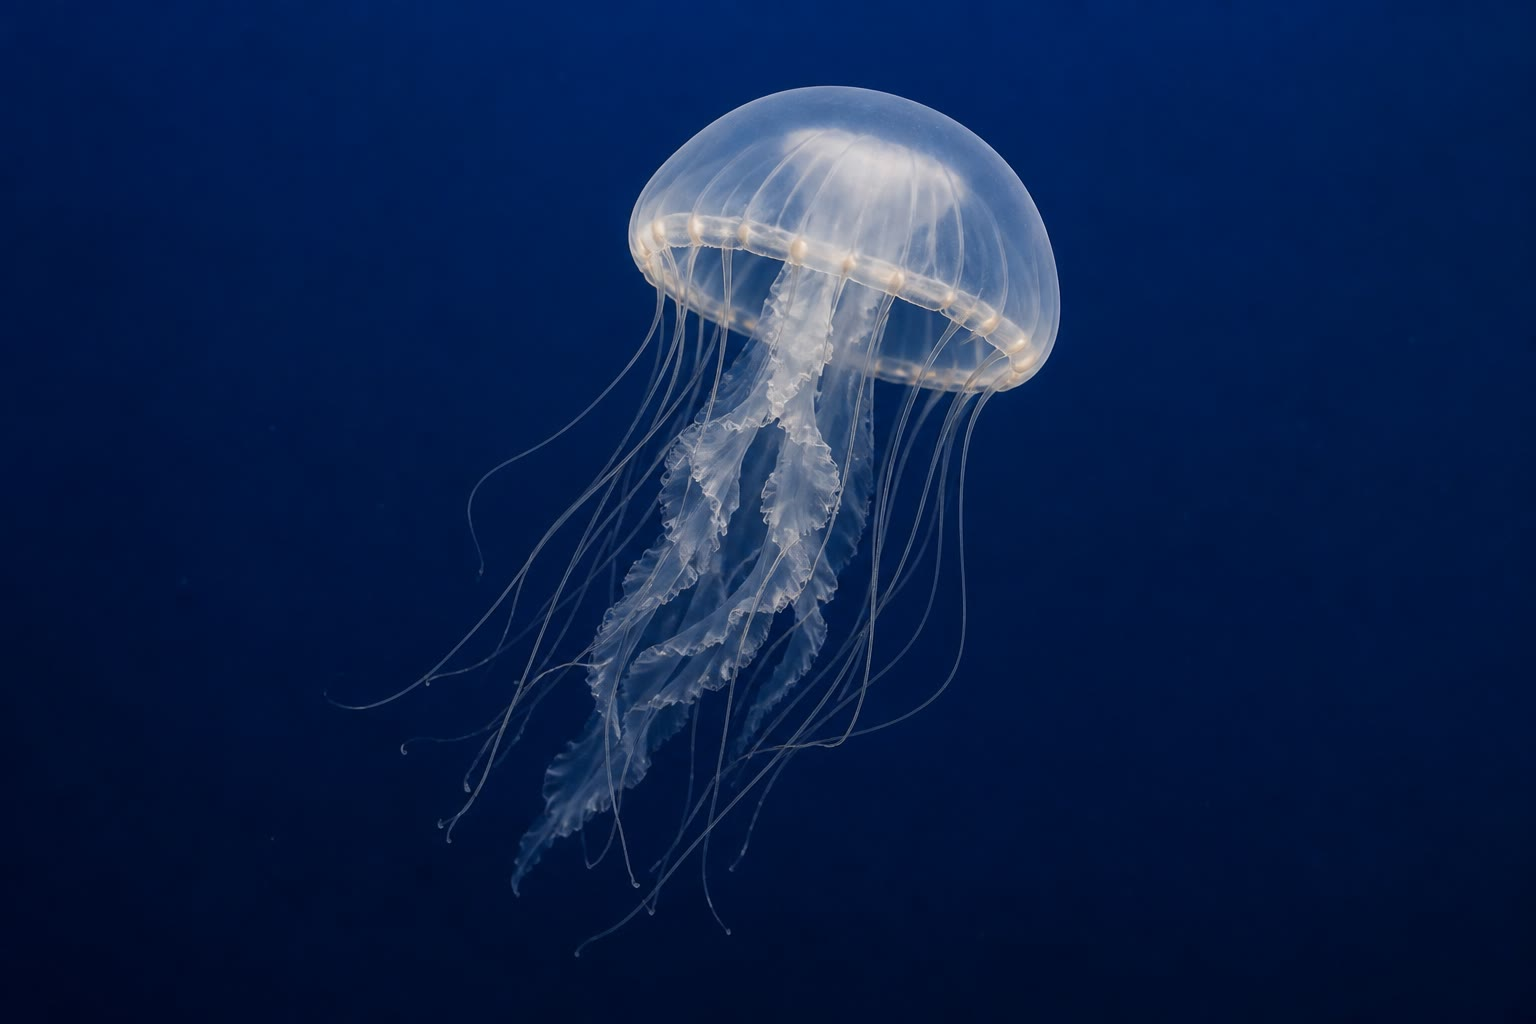
\includegraphics[width=0.46\linewidth]{images/book5/ai/b5-17-jellyfish.jpg}\hspace{0.04\linewidth}
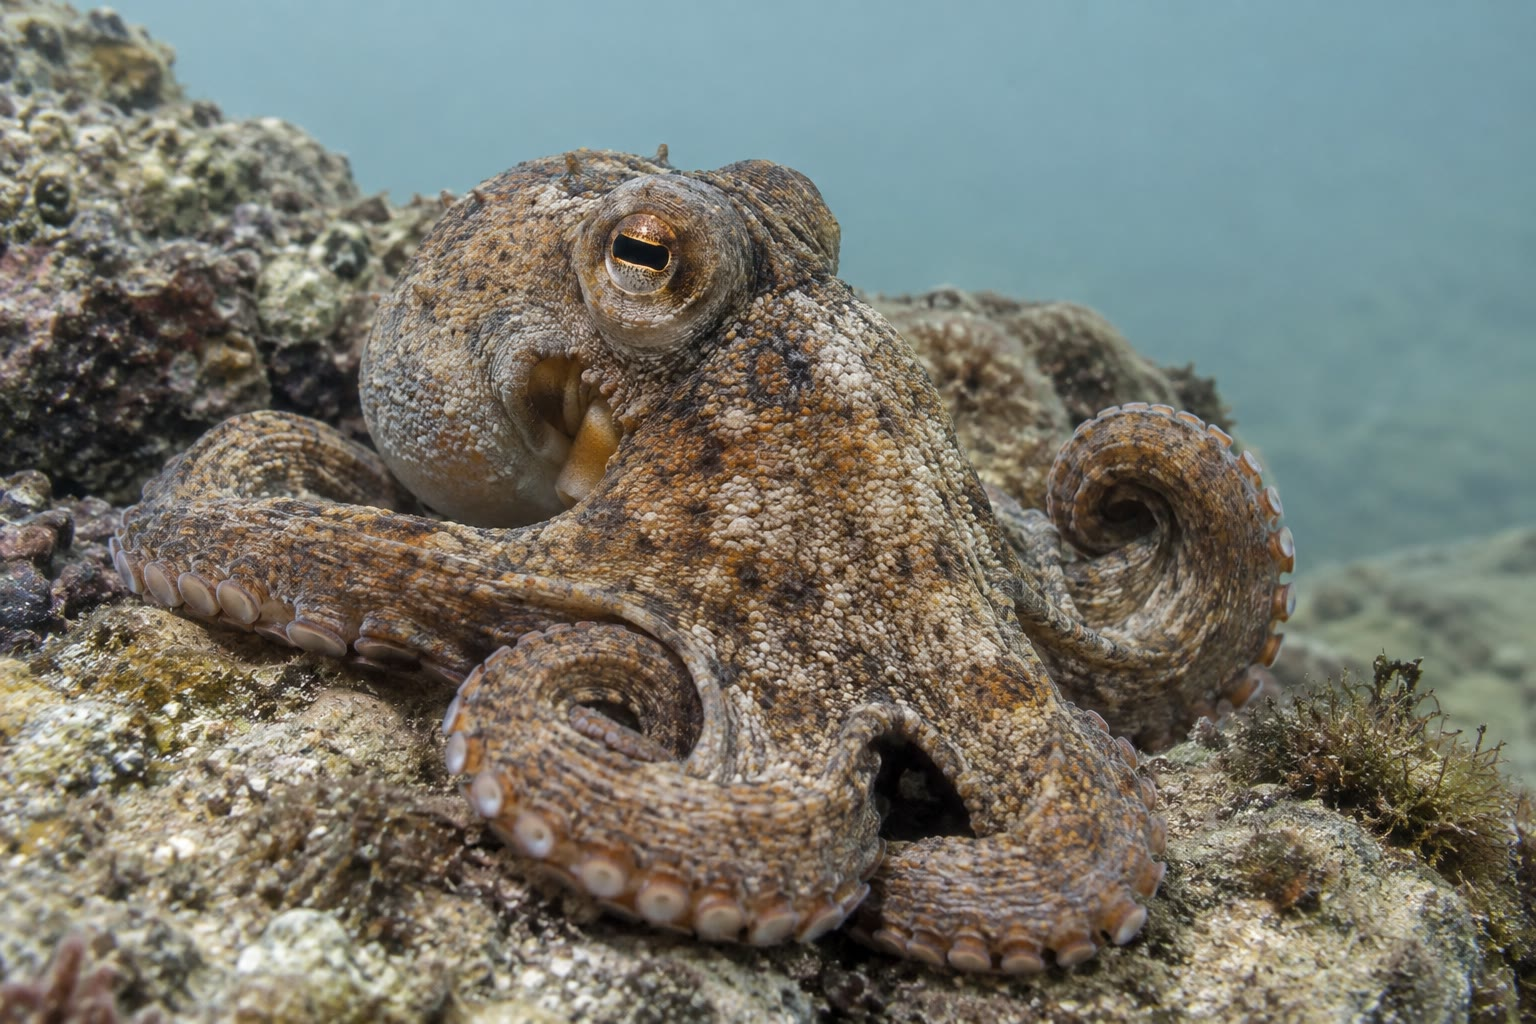
\includegraphics[width=0.46\linewidth]{images/book5/ai/b5-17-octopus.jpg}

{\small Deux façons d'organiser des neurones. À gauche~: une méduse,
dont le \omterm{def:b3:nervous-systems:comparative}{réseau nerveux diffus} et les anneaux marginaux coordonnent la
nage sans cerveau. À droite~: une pieuvre, avec un demi-milliard de
neurones, la plupart dans les bras, et le plus grand cerveau de tous les
invertébrés.}
\end{omfigure}

\begin{remark}[À quoi sert un système nerveux]\label{rem:b3:nervous-systems:for}
Les plantes, les champignons et les éponges n'en ont aucun~; un animal
qui se déplace en a besoin, et l'élaboration des systèmes nerveux suit
les exigences du mouvement, de la perception à distance et de la
prédiction de ce qui va arriver. L'\omterm{thm:b3:nervous-systems:cable}{équation du câble} fixe la physique
--- jusqu'où et à quelle vitesse un signal chemine pour un diamètre et
une isolation donnés~; le budget énergétique fixe l'économie~; et dans
ces limites les mêmes neurones, arrangés en réseaux, en \omterm{def:b3:nervous-systems:comparative}{ganglions} ou en
cortex, produisent la pulsation d'une méduse, le camouflage d'une
pieuvre ou cette phrase. Les deux chapitres suivants prennent le bout
d'entrée et le stockage~: comment les sens transforment le monde en
potentiels, et comment les synapses changent pour que le monde, une fois
rencontré, soit retenu.
\end{remark}

\section{Exercices}

\begin{exercise}[$\star$]\label{exo:b3:nervous-systems:1}
Nommer les quatre sortes de \omterm{def:b3:nervous-systems:cells}{glie} et une fonction de chacune, et dire
lesquelles d'entre elles fabriquent la \omterm{def:b3:nervous-systems:cells}{myéline} et où.
\end{exercise}

\begin{exercise}[$\star$]\label{exo:b3:nervous-systems:2}
Qu'a permis l'imprégnation de Golgi, qu'en a conclu Cajal, et qu'en a
conclu Golgi~? Qui avait raison, et comment cela fut-il tranché~?
\end{exercise}

\begin{exercise}[$\star$]\label{exo:b3:nervous-systems:3}
Décrire l'\omterm{def:b3:nervous-systems:circuits}{arc réflexe} rotulien et expliquer pourquoi il ne prend que
\qty{30}{ms} alors qu'un coup de pied volontaire prend dix fois plus.
\end{exercise}

\begin{exercise}[$\star$]\label{exo:b3:nervous-systems:4}
Énumérer les effets sympathiques et parasympathiques sur le cœur, la
pupille, l'intestin et les voies aériennes, et le transmetteur que
chaque division emploie à la cible.
\end{exercise}

\begin{exercise}[$\star\star$]\label{exo:b3:nervous-systems:5}
Calculer la \omterm{thm:b3:nervous-systems:cable}{constante d'espace} d'un axone de \qty{1}{\micro m} avec $R_{m}
= \qty{1e4}{\ohm.cm^2}$ et $R_{i} = \qty{100}{\ohm.cm}$, et la fraction
d'un signal qui subsiste après \qty{2}{mm}. Quel diamètre doublerait
$\lambda$~?
\end{exercise}

\begin{exercise}[$\star\star$]\label{exo:b3:nervous-systems:6}
Un axone sensoriel de \qty{12}{\micro m} court sur \qty{1.2}{m} de
l'orteil à la moelle, et un axone moteur de \qty{15}{\micro m} revient.
Avec \qty{6}{m/s} par micromètre et \qty{0.5}{ms} par synapse, estimer
la latence minimale d'un réflexe spinal de retrait à un \omterm{def:b3:nervous-systems:cells}{interneurone}.
Combien de temps cela prendrait-il avec des axones amyéliniques de même
diamètre à $v = 1.1\sqrt{d}$~?
\end{exercise}

\begin{exercise}[$\star\star$]\label{exo:b3:nervous-systems:7}
À l'aide du budget du cerveau de la
\cref{prop:b3:nervous-systems:barrier-budget}, estimer combien d'ATP un
neurone peut dépenser par seconde et, si un potentiel avec ses synapses
coûte $2\times 10^{9}$ ATP, la fréquence de décharge moyenne que le
budget autorise. Que cela prédit-il du code~?
\end{exercise}

\begin{exercise}[$\star\star$]\label{exo:b3:nervous-systems:8}
Expliquer pourquoi un \omterm{prop:b3:nervous-systems:cpg}{oscillateur à demi-centres} a besoin d'une fatigue
(ou d'un autre processus lent) pour osciller, et ce qui arriverait avec
deux neurones s'inhibant mutuellement qui ne se fatigueraient jamais.
\end{exercise}

\begin{exercise}[$\star\star$]\label{exo:b3:nervous-systems:9}
La \omterm{prop:b3:nervous-systems:barrier-budget}{barrière hémato-encéphalique} exclut la dopamine, produit de la
L-dopa, mais admet la L-dopa. Expliquer comment on l'exploite dans la
maladie de Parkinson et pourquoi les \omterm{def:b3:adaptive-immunity:antibody}{anticorps} dirigés contre des
protéines cérébrales sont difficiles à livrer.
\end{exercise}

\begin{exercise}[$\star\star\star$]\label{exo:b3:nervous-systems:10}
Établir la forme dépendante du temps de l'\omterm{thm:b3:nervous-systems:cable}{équation du câble},
$\lambda^{2}\,\partial^{2}
V/\partial x^{2} = \tau\,\partial V/\partial t + V$, en ajoutant le
courant capacitif au courant membranaire, et montrer que la solution
stationnaire du théorème s'ensuit. (Donner la forme~; il n'est pas
demandé de la résoudre.) Pourquoi le rapport $\lambda/\tau$ est-il une
vitesse~?
\end{exercise}

\begin{exercise}[$\star\star\star$]\label{exo:b3:nervous-systems:11}
Un axone géant de calmar de \qty{500}{\micro m} conduit à \qty{25}{m/s}.
En utilisant $v \propto \sqrt{d}$, quel diamètre d'axone amyélinique
faudrait-il pour \qty{100}{m/s}~? Calculer l'aire de la section et
comparer à l'axone myélinisé de \qty{20}{\micro m} qui y parvient. Qu'en
déduire sur le nombre de fibres rapides qu'un nerf peut porter, et sur
l'évolution de la \omterm{def:b3:nervous-systems:cells}{myéline}~?
\end{exercise}

\begin{exercise}[$\star\star\star$]\label{exo:b3:nervous-systems:12}
La masse du cerveau varie comme $M_{\text{corps}}^{0.75}$ chez les
mammifères. Une souris de \qty{30}{g} a un cerveau de \qty{0.4}{g}.
Prévoir la masse du cerveau d'un mammifère de \qty{70}{kg} sur la
droite, comparer aux \qty{1350}{g} de l'humain, et discuter pourquoi le
nombre de neurones corticaux plutôt que la masse du cerveau est le
meilleur corrélat de la capacité cognitive.
\end{exercise}

\section{Problème~: câbler un corps}

\begin{problem}[{Problème du week-end --- le câblage d'un corps chiffré
en constantes d'espace, en millisecondes et en watts~: les nombres du
câble d'une dendrite et de deux axones, la latence d'un réflexe de
l'orteil à la moelle et retour, l'énergie que le cerveau peut consacrer
à chaque potentiel, et la mise à l'échelle des cerveaux entre animaux,
pour finir sur la constante d'espace, la latence du réflexe et la
fréquence de décharge moyenne qu'un cerveau peut payer}]
\label{pb:b3:nervous-systems:1}
Données~: $R_{m} = \qty{2e4}{\ohm.cm^2}$, $R_{i} = \qty{100}{\ohm.cm}$,
$C_{m} = \qty{1}{\micro F/cm^2}$. Vitesse myélinisée \qty{6}{m/s} par
micromètre~; amyélinique $v = 1.1\sqrt{d}$ m/s avec $d$ en
micromètres~; délai synaptique \qty{0.5}{ms}. Cerveau~: \qty{20}{W},
$8.6\times 10^{10}$ neurones, $10^{14}$ synapses, ATP \qty{50}{kJ/mol}~;
un potentiel coûte $4\times 10^{8}$ ATP et chaque transmission
synaptique $2\times 10^{4}$ ATP~; un neurone a \num{7000} synapses. Mise
à l'échelle~: $M_{\text{cerveau}} = a\,M_{\text{corps}}^{0.75}$ avec une
souris de \qty{30}{g} ayant un cerveau de \qty{0.4}{g}.

\medskip
\noindent\textbf{Partie I --- Les câbles.}
\begin{enumerate}
  \item Calculer $\lambda$ pour des dendrites de \qty{1}{\micro m} et de
        \qty{4}{\micro m}, et $\tau$.
  \item Une synapse à \qty{300}{\micro m} du soma sur la dendrite de
        \qty{1}{\micro m} produit \qty{5}{mV} localement. Qu'arrive-t-il
        au soma~? Sur la dendrite de \qty{4}{\micro m}~?
  \item Expliquer pourquoi un neurone peut pondérer ses entrées selon
        l'endroit de l'arbre où elles se posent, et pourquoi les entrées
        doivent arriver en moins de $\tau$ environ pour se sommer.
  \item Calculer la vitesse d'un axone myélinisé de \qty{10}{\micro m},
        et celle d'un axone amyélinique de même diamètre. Quel diamètre
        d'axone amyélinique égalerait le myélinisé~?
  \item Aires des sections de l'axone de \qty{10}{\micro m} et de
        l'équivalent amyélinique. Combien d'axones myélinisés tiennent
        dans la place d'un seul axone amyélinique équivalent~?
  \item Une maladie démyélinisante retire la \omterm{def:b3:nervous-systems:cells}{myéline} d'un axone de
        \qty{10}{\micro m} sur \qty{2}{cm}. Estimer le délai
        supplémentaire sur ce tronçon s'il conduit comme un axone
        amyélinique de ce diamètre, et dire pourquoi la conduction peut
        échouer tout à fait.
\end{enumerate}

\medskip
\noindent\textbf{Partie II --- Les latences.}
\begin{enumerate}[resume]
  \item Un orteil touche une surface brûlante. L'axone sensoriel
        (\qty{10}{\micro m}, \qty{1.2}{m}) atteint la moelle, un
        \omterm{def:b3:nervous-systems:cells}{interneurone}, et un axone moteur (\qty{15}{\micro m},
        \qty{1.1}{m}) revient à la jambe. Latence minimale du retrait~?
  \item Le signal remonte aussi un axone de \qty{10}{\micro m} sur
        \qty{0.6}{m} jusqu'au cerveau et franchit deux synapses de plus
        avant que la douleur soit ressentie. Quand la douleur est-elle
        ressentie par rapport au retrait~?
  \item Une fibre de la douleur est amyélinique, \qty{1}{\micro m}.
        Combien de temps son signal met-il à parcourir les \qty{1.8}{m}
        jusqu'au cerveau~? Expliquer les deux temps de la douleur d'un
        orteil cogné.
  \item La jambe d'une girafe est plus longue de \qty{2}{m}. Recalculer
        la latence du réflexe et commenter les problèmes de la taille.
  \item Le réflexe rotulien est monosynaptique, \qty{30}{ms} chez
        l'adulte. Avec \qty{0.8}{m} à l'aller comme au retour à
        \qty{80}{m/s}, une synapse et une jonction neuromusculaire
        (\qty{1}{ms}), et \qty{5}{ms} pour que le muscle développe sa
        force, rendre compte des \qty{30}{ms}.
  \item Les axones d'un nouveau-né sont amyéliniques. Expliquer pourquoi
        ses réflexes sont lents et ses mouvements mal coordonnés, et ce
        que change la myélinisation des deux premières années.
\end{enumerate}

\medskip
\noindent\textbf{Partie III --- Le budget.}
\begin{enumerate}[resume]
  \item Convertir \qty{20}{W} en ATP par seconde, et en ATP par neurone
        et par seconde.
  \item Un neurone émet un potentiel~: il coûte $4\times 10^{8}$ ATP à
        lui seul et commande \num{7000} synapses à $2\times 10^{4}$
        chacune. Coût total d'un potentiel avec ses conséquences~?
  \item Quelle fréquence de décharge moyenne le budget soutient-il si
        tout y passait~? Et si la moitié va aux coûts de repos~?
  \item Les neurones corticaux déchargent à environ \qty{1}{Hz} en
        moyenne. Quelle fraction du budget cela fait-il, et qu'en
        déduire sur la façon dont l'information est codée~?
  \item Un cerveau qui ferait décharger chaque neurone à \qty{50}{Hz}
        demanderait combien de watts~? Comparer aux \qty{100}{W} du
        corps entier.
  \item Le glucose alimente le cerveau à \qty{5}{g/h}. Combien de watts
        cela fait-il (\qty{16}{kJ/g})~? Est-ce assez, et qu'advient-il de
        la conscience en quelques secondes si l'apport s'arrête~?
\end{enumerate}

\medskip
\noindent\textbf{Partie IV --- La mise à l'échelle.}
\begin{enumerate}[resume]
  \item Trouver $a$ à partir de la souris, puis prévoir la masse du
        cerveau d'un mammifère de \qty{70}{kg} et d'un éléphant de
        \qty{5000}{kg} sur la droite.
  \item Valeurs réelles~: humain \qty{1350}{g}, éléphant \qty{4800}{g}.
        Calculer pour chaque espèce le rapport à la prévision (le
        quotient d'\omterm{def:b3:nervous-systems:comparative}{encéphalisation}).
  \item Le cerveau de l'éléphant a $2.6\times 10^{11}$ neurones mais
        $5.6\times 10^{9}$ dans le cortex~; l'humain $8.6\times 10^{10}$
        et $1.6\times 10^{10}$. Où sont les neurones de l'éléphant, et
        qu'est-ce que cela suggère de ce que fait le cortex~?
  \item Le volume d'un neurone croît avec la longueur de son axone, de
        sorte que les gros cerveaux ont des neurones plus gros et plus
        clairsemés. Expliquer pourquoi doubler la masse du cerveau ne
        double pas le nombre de neurones, et pourquoi les primates, dont
        les neurones restent petits quand le cerveau grossit, gagnent
        plus de neurones par gramme que les rongeurs.
  \item Une pieuvre a $5\times 10^{8}$ neurones, les deux tiers dans ses
        bras. Proposer ce qu'un bras peut et ne peut pas faire sans le
        cerveau, et une expérience pour le vérifier.
  \item Le nématode \emph{C.~elegans} a $302$ neurones et environ
        \num{7000} synapses en tout, toutes cartographiées. Comparer son
        nombre de synapses par neurone au chiffre humain, et dire ce
        qu'un schéma de câblage complet peut et ne peut pas nous
        apprendre du comportement.
  \item Résumer~: la \omterm{thm:b3:nervous-systems:cable}{constante d'espace} de la dendrite de
        \qty{1}{\micro m} (question~1), la latence du réflexe de retrait
        (question~7), et la fréquence de décharge moyenne que le budget
        du cerveau autorise avec la moitié de son énergie aux potentiels
        (question~15).
\end{enumerate}
\end{problem}
